\section{Regression accuracy}
This section includes an examination of the accuracy of the regressors. This will be examined through superimposition of the regressor outputs on the estimated data, and through RMSE plots. To evaluate how the regressors performed they were given a test data set as input to examine the accuracy of the trained regressors. Ths test data set consisted of the 50\% contraction recording and were performed for all movements in all limb positions. \\

\begin{figure}[H]
	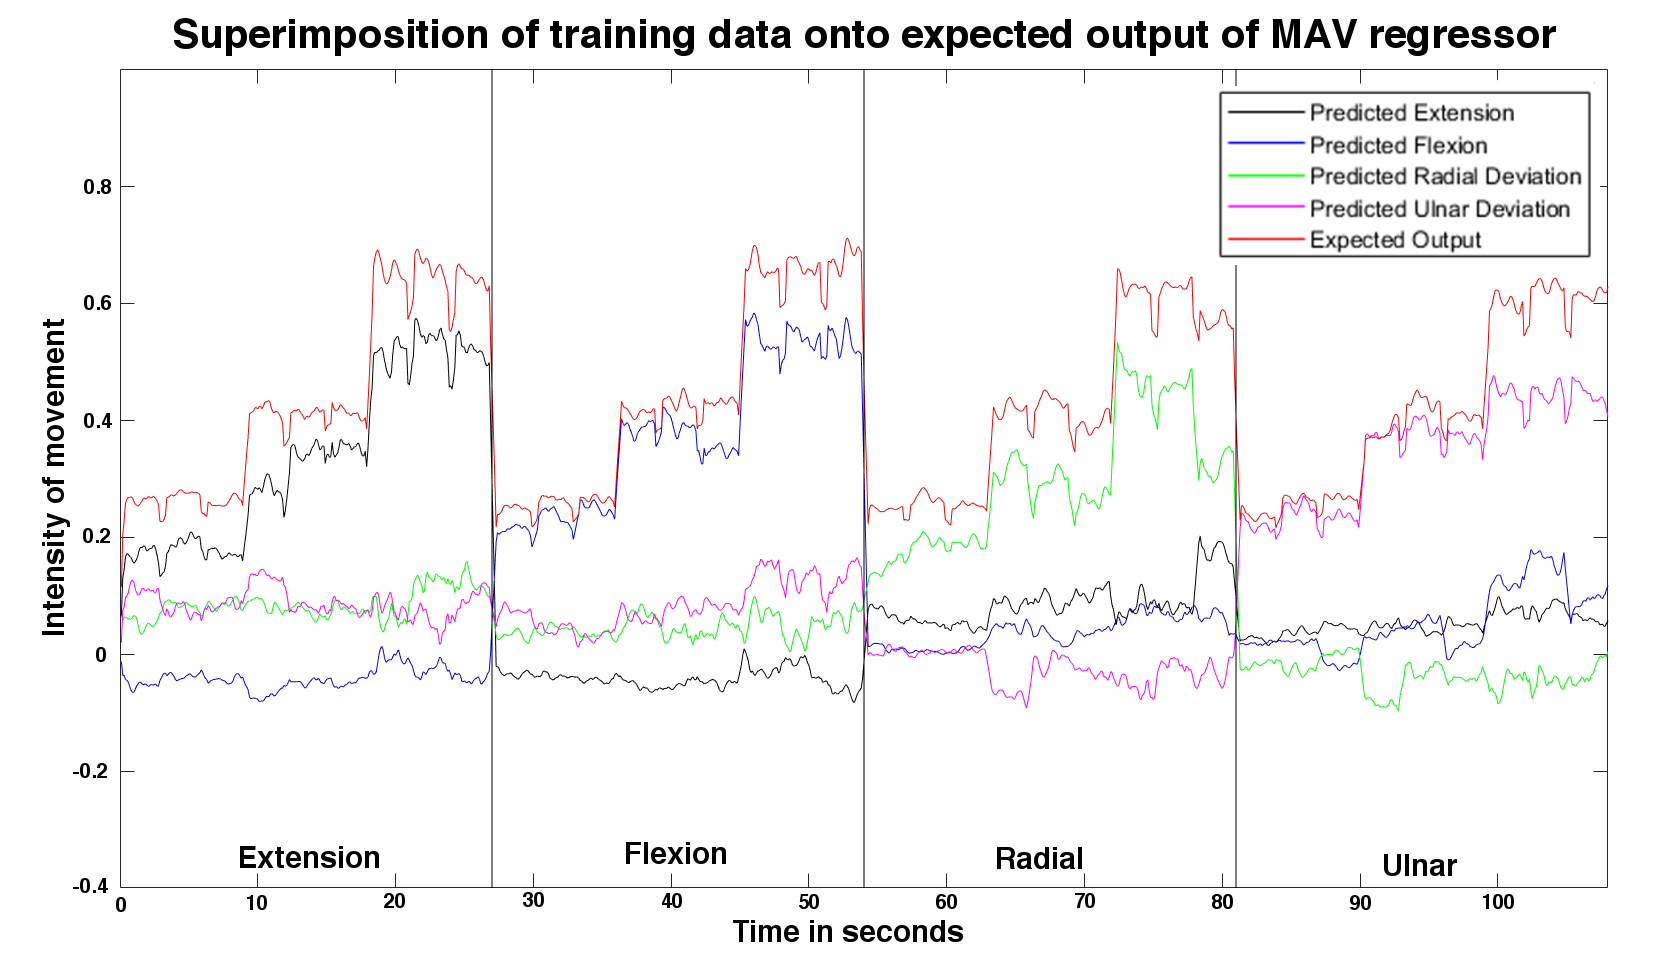
\includegraphics[width=1\textwidth]{figures/results/NewSuperPositionTestDataMAV}  %<--but is not needed.
	\caption{Plot of the expected data, red plot, superimposed on the output of the regressors trained with the MAV feature. The plot is divided into four segments, where each segment shows a different movement performed. Each segment has the same sample size.}
	\label{fig:SuperPositionTestDataMAV}  %<--give the figure a label, so you can reference!
\end{figure}
The plot in \figref{fig:SuperPositionTestDataMAV} depicts the actual data superimposed on the estimated data from the regressors trained with the MAV features. 

\begin{figure}[H]
	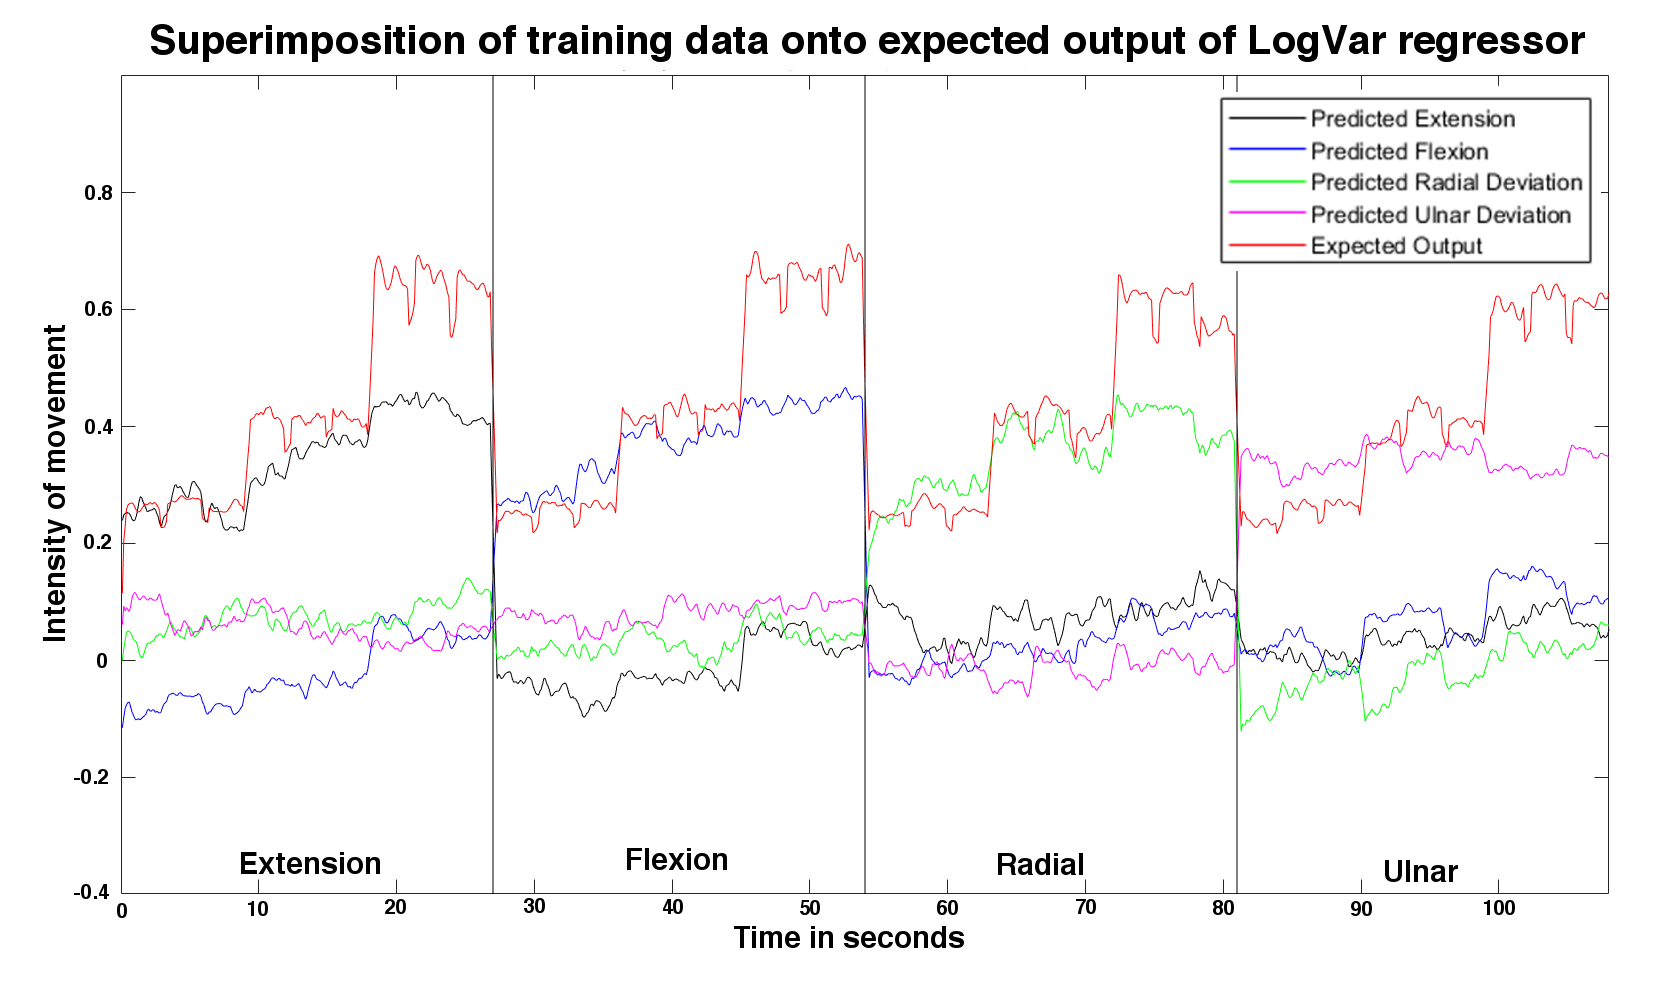
\includegraphics[width=1\textwidth]{figures/results/NewSuperPositionTestDataLogVar}  %<--but is not needed.
	\caption{Plot of the expected data, red plot, superimposed on the output of the regressors trained with the LogVar feature. The plot is divided into four segments, where each segment shows a different movement performed. Each segment has the same sample size.}
	\label{fig:SuperPositionTestDataLogVar}  %<--give the figure a label, so you can reference!
\end{figure}
The plot in \figref{fig:SuperPositionTestDataLogVar} depicts the actual data superimposed on the estimated data from the regressors trained with the LogVar features. 

A qualitative examination of the plots depicted in \figref{fig:SuperPositionTestDataLogVar} and \figref{fig:SuperPositionTestDataMAV} shows that each regressor reacts on the movement it is fitted for, and remains inactive when another movement is performed. This accounts for both features. Both regressors has a lower accuracy in the high intensities though, especially for the regressors trained with logarithmic variance features. It is also seen that regressor fitted for the antagonistic movement is more inactive than the other regressors, when the other movement representing that DOF is performed. Furthermore, the regressor output is lower in intensity in all movements above 30\% of the MVC. 
%regression on MAV features yields a more accurate output than regression on the logarithmic variance feature, whereas both estimates yield inaccurate fitting in the high intensities. However, both estimates yield inaccurate fitting in the high intensities compared to the lower intensities, especially in the ulnar deviation movement.
Calculating the RMSE of the regressors for the MAV and LogVar features of the training data across all subjects, yields the results depicted in \figref{fig:gimmeThemRMSEBars}. 

\begin{figure}[H]
	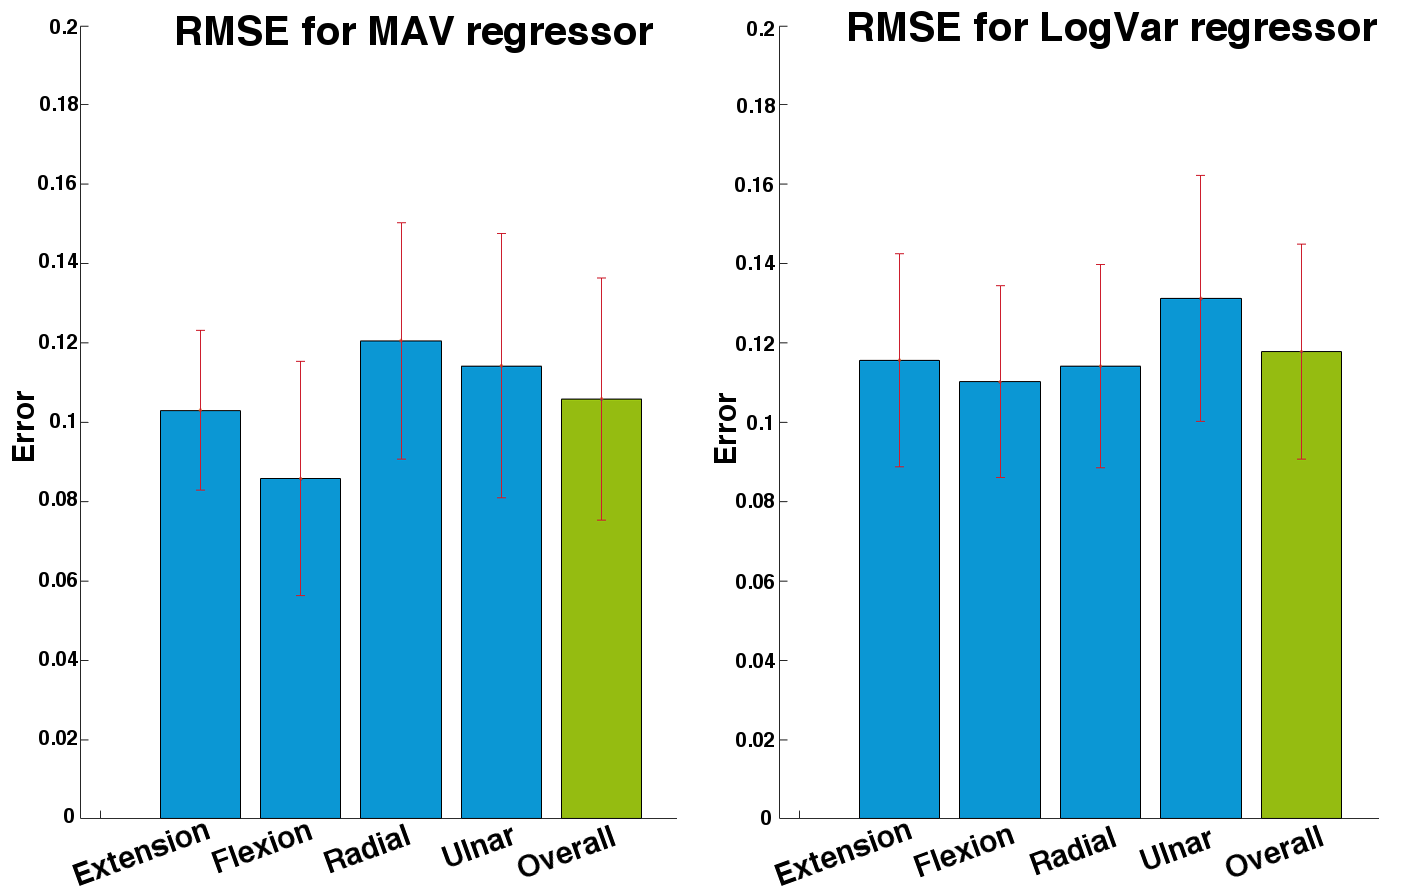
\includegraphics[width=1\textwidth]{figures/results/gimmeThemRMSEBars}  %<--but is not needed.
	\caption{Bar plot of the mean error of MAV and the LogVar features for the four hand gestures. The bar chart illustrates the mean error and the error bar illustrates the standard deviation.}
	\label{fig:gimmeThemRMSEBars}  %<--give the figure a label, so you can reference!
\end{figure}

	\begin{center}
		\begin{tabular}{l l l}
			\toprule
			\textbf{Feature} & \textbf{Overall mean error} & \textbf{Standard deviation}\\
			\midrule
			Extension & 0.10 & $\pm 0.02$ \\
			Flexion & 0.11 & $\pm 0.03$ \\
			Radial Deviation & 0.12 & $\pm 0.03$ \\
			Ulnar Deviation & 0.11 & $\pm 0.03$ \\
			Overall & 0.11 & $\pm 0.03$ \\
			\bottomrule
		\end{tabular}
		\captionof{table}{RMSE for the implemented MAV regressor.}
	\end{center}
	
	\begin{center}
		\begin{tabular}{l l l}
			\toprule
			\textbf{Feature} & \textbf{Overall mean error} & \textbf{Standard deviation}\\
			\midrule
			Extension & 0.12 & $\pm 0.05$ \\
			Flexion & 0.11 & $\pm 0.02$ \\
			Radial Deviation & 0.11 & $\pm 0.03$ \\
			Ulnar Deviation & 0.13 & $\pm 0.03$ \\
			Overall & 0.12 & $\pm 0.03$ \\
			\bottomrule
		\end{tabular}
		\captionof{table}{RMSE for the implemented LogVar regressor.}
	\end{center}

The overall mean of the RMSE of MAV is 0.09 with a standard deviation of $\pm 0.03$, where the highest mean of a regressor is 0.12 and the highest standard deviation is $\pm 0.04$. The overall mean of the RMSE of LogVar is 0.11 with a standard deviation of $\pm 0.03$, where the highest mean of a regressor is 0.12 and the highest standard deviation is $\pm 0.04$. MAV then yields a lower mean RMSE and a lower standard deviation than LogVar - both with the overall RMSE and for the movement with the highest RMSE.

\subsection{Accuracy of regressors with test data}
This section contains the superimposition of the expected output of the regressors on the output of the regressors with test data. The plot in \figref{fig:SuperPoisonLogVarNewData} depicts the superimposition the logarithmic variace trained regressors fed with the test data.

\begin{figure}[H]
	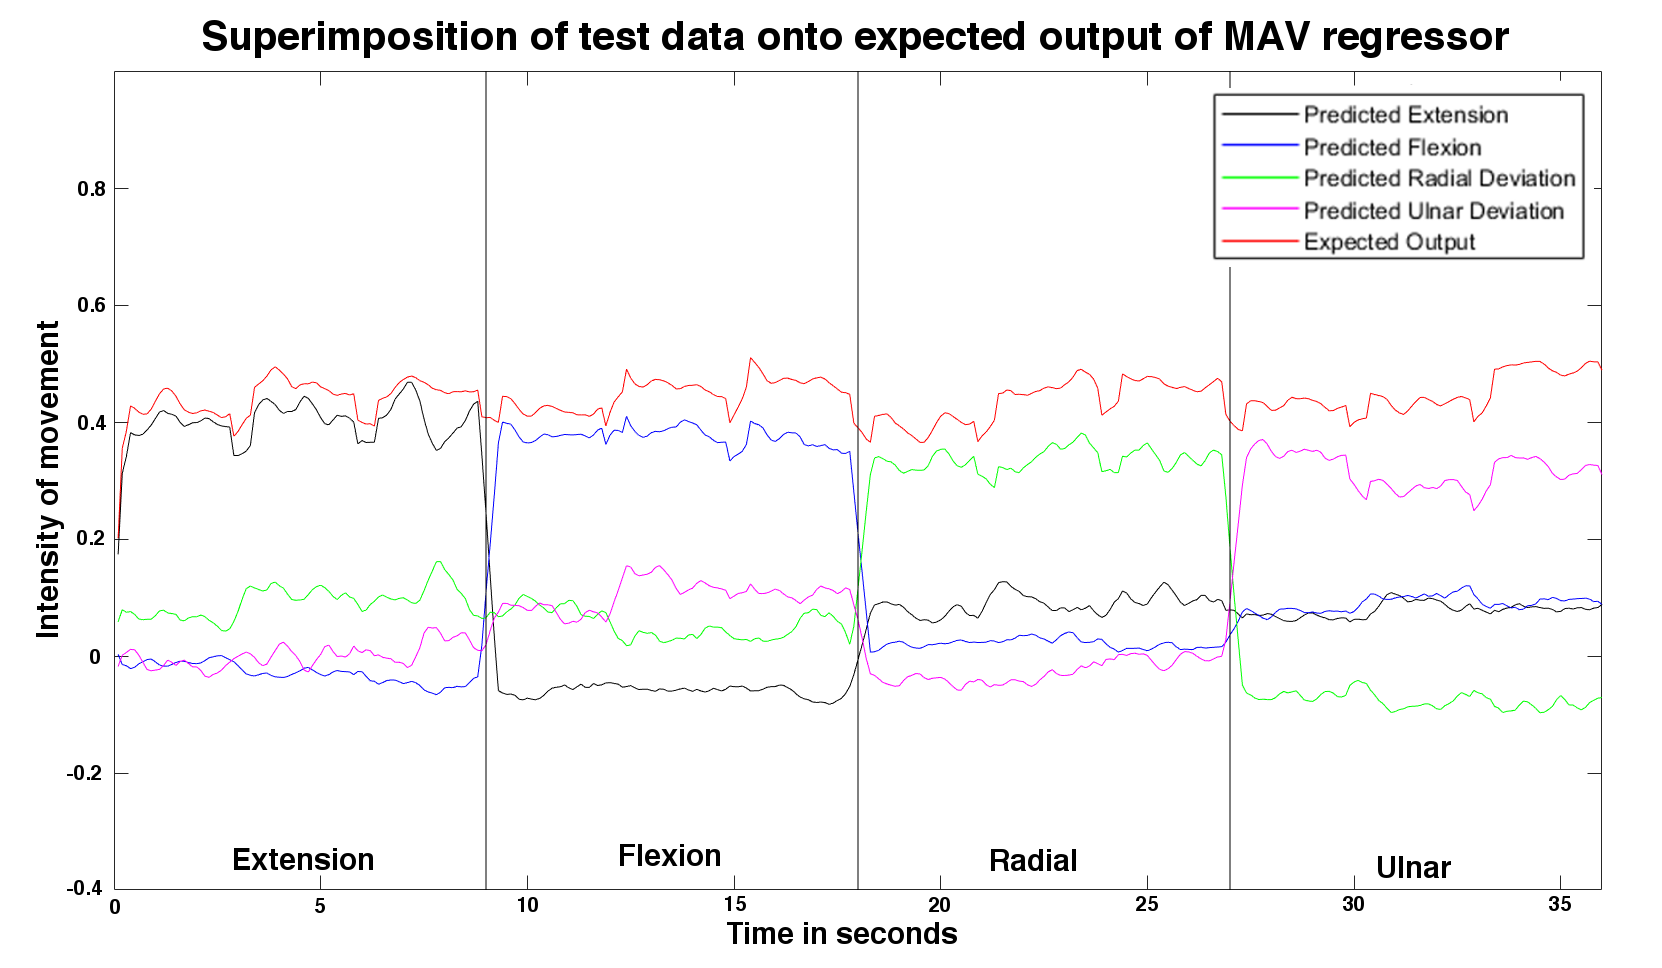
\includegraphics[width=1\textwidth]{figures/results/NewSuperPoisonMavNewData}  %<--but is not needed.
	\caption{Plot of the expected output (red plot) for the regressors trained with the MAV feature , superimposed on the output of the regressors where 50\% contraction test data is given as input. The plot is divided into four segments, where each segment shows a different movement performed. Each segment has the same sample size.}
	\label{fig:SuperPoisonMavNewData}  %<--give the figure a label, so you can reference!
\end{figure}

\begin{figure}[H]
	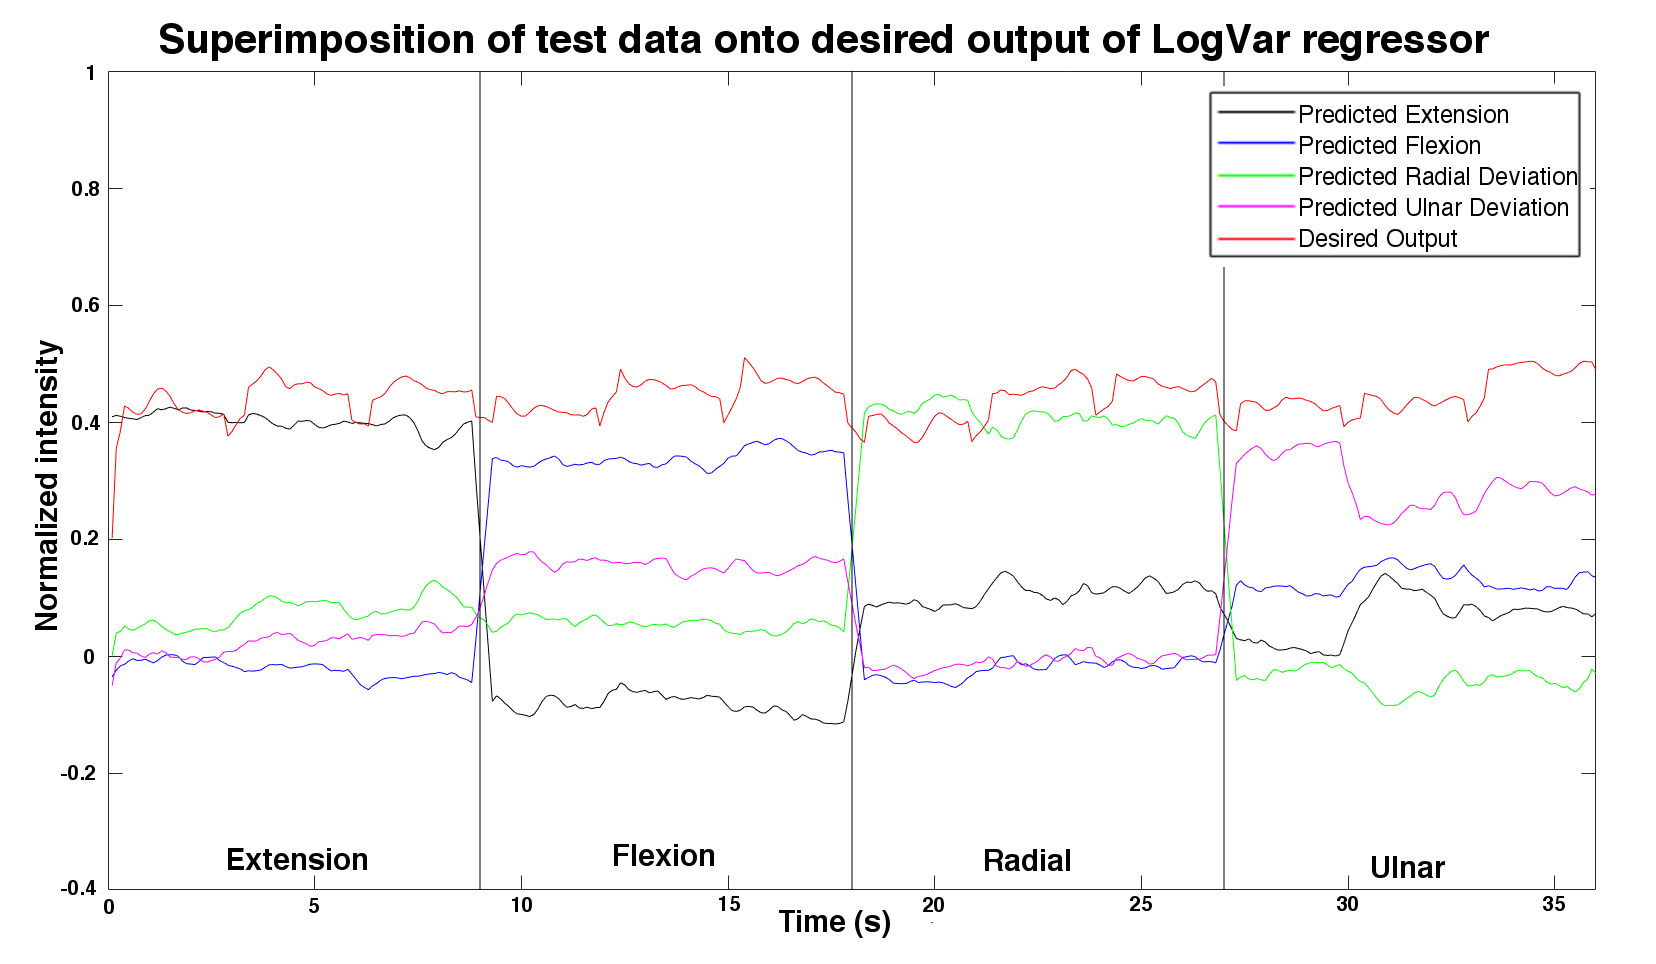
\includegraphics[width=1\textwidth]{figures/results/NewSuperPoisonLogVarNewData}  %<--but is not needed.
	\caption{Plot of the expected output (red plot) for the regressors trained with the LogVar feature , superimposed on the output of the regressors where 50\% contraction test data is given as input. The plot is divided into four segments, where each segment shows a different movement performed. Each segment has the same sample size.}
	\label{fig:SuperPoisonLogVarNewData}  %<--give the figure a label, so you can reference!
\end{figure}

The superimpositions in \figref{fig:SuperPoisonMavNewData} and \figref{fig:SuperPoisonLogVarNewData} show a similar pattern as the superimpositions for the output of the regressors given training data as input, but with a higher error. 

\begin{figure}[H]
	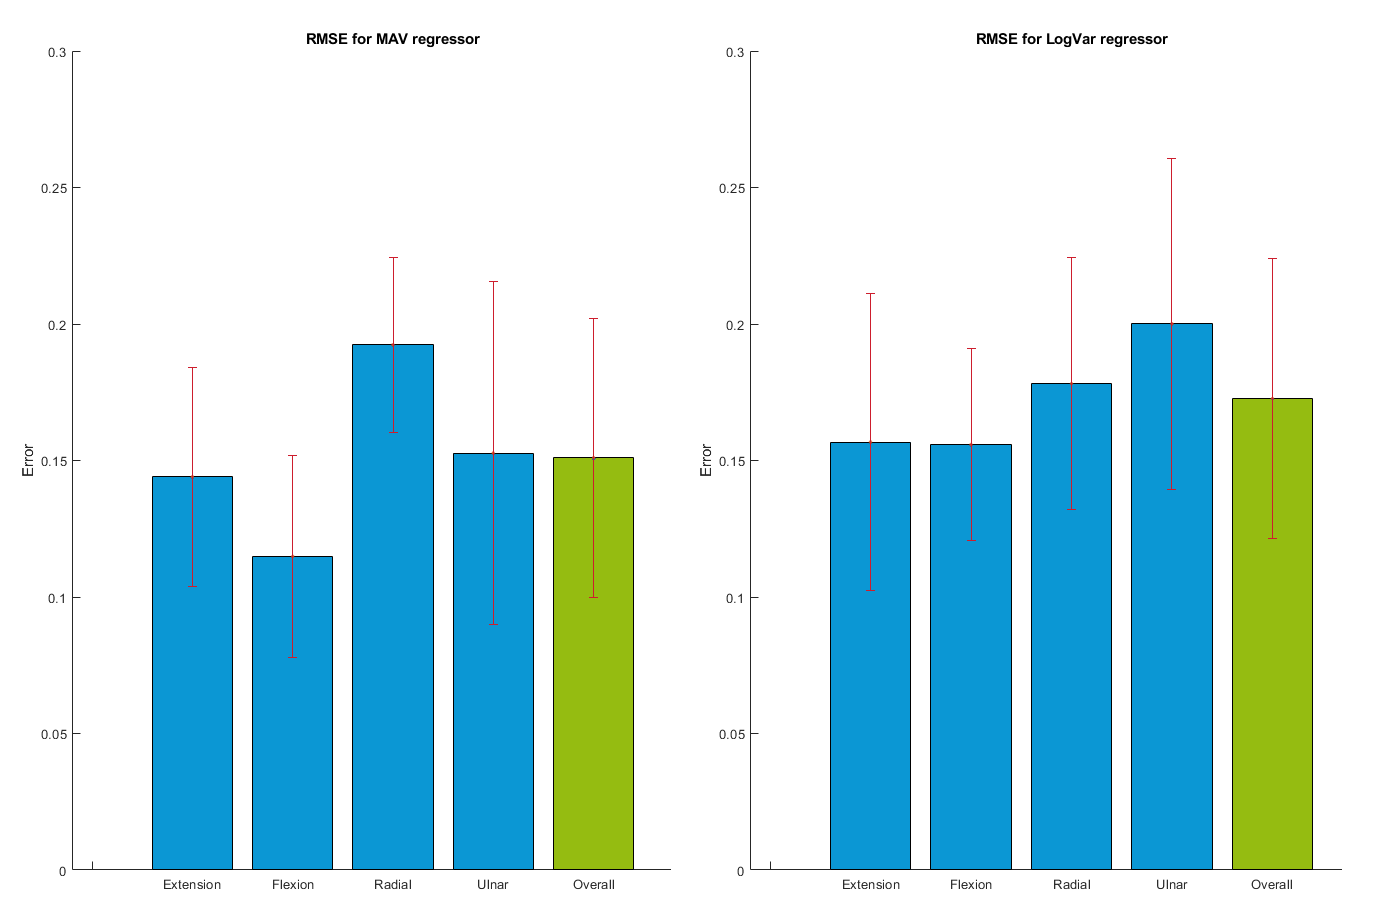
\includegraphics[width=1\textwidth]{figures/results/RMSEBarPlotNewData}  %<--but is not needed.
	\caption{Bar plot of the mean error of the MAV and LogVar features for the four hand gestures when the regressors are given test data as input. The bar chart illustrates the mean error and the error bar illustrates the standard deviation.}
	\label{fig:RMSEBarPlotNewData}  %<--give the figure a label, so you can reference!
\end{figure}

	\begin{center}
		\begin{tabular}{l l l}
			\toprule
			\textbf{Feature} & \textbf{Overall mean error} & \textbf{Standard deviation}\\
			\midrule
			Extension & 0.14 & $\pm 0.04$ \\
			Flexion & 0.11 & $\pm 0.04$ \\
			Radial Deviation & 0.19 & $\pm 0.03$ \\
			Ulnar Deviation & 0.15 & $\pm 0.06$ \\
			Overall & 0.15 & $\pm 0.05$ \\
			\bottomrule
		\end{tabular}
		\captionof{table}{RMSE for the implemented MAV regressor.}
	\end{center}
	

	
	\begin{center}
		\begin{tabular}{l l l}
			\toprule
			\textbf{Feature} & \textbf{Overall mean error} & \textbf{Standard deviation}\\
			\midrule
			Extension & 0.16 & $\pm 0.05$ \\
			Flexion & 0.16 & $\pm 0.04$ \\
			Radial Deviation & 0.18 & $\pm 0.05$ \\
			Ulnar Deviation & 0.20 & $\pm 0.06$ \\
			Overall & 0.17 & $\pm 0.05$ \\
			\bottomrule
		\end{tabular}
		\captionof{table}{RMSE for the implemented LogVar regressor.}
	\end{center}
	
		\begin{center}
			\begin{tabular}{l l}
				\toprule
				\textbf{Feature} & \textbf{P-Value}\\
				\midrule
				LogVar and MAV & < 0.01 \\
				LogVar new data and MAV new data & 0.1138 \\
				LogVar new data and LogVar & < 0.001 \\
				MAV new data and MAV & < 0.001 \\
				\bottomrule
			\end{tabular}
			\captionof{table}{P-Values for comparison of the features.}
		\end{center}
		
A Friedman's statistical test showed a significant difference (p < 0.01) between the RMSE for the MAV and LogVar regressors with the training data as input, where LogVar has the higher mean. When examining the RMSE for the regressors with test data, showed that there is no significant difference (p = 0.1138) between the offline performance of the two regressors. When comparing the offline tests with training data and 50\% test data, it was shown that there's a significant difference for both LogVar (p < 0.001) and LogVar (p < 0.001), where the mean is higher for when setting the test data as input.